\documentclass[residuals.tex]{subfiles}
\begin{document}
\Large	
\section{mtcars example} %Ready 1

\textit{Several data sets , intended as learning tools, are automatically installed when \texttt{R} is installed. Many more are installed within packages to complement learning to use those packages. One of these is the famous \textbf{\textit{mtcars}} data set, which is used in many data mining exercises.}
{
	\large
\begin{framed}
\begin{verbatim}
> data(mtcars)
> head(mtcars)
                   mpg cyl disp  hp drat    wt  qsec vs am gear carb
Mazda RX4         21.0   6  160 110 3.90 2.620 16.46  0  1    4    4
Mazda RX4 Wag     21.0   6  160 110 3.90 2.875 17.02  0  1    4    4
Datsun 710        22.8   4  108  93 3.85 2.320 18.61  1  1    4    1
Hornet 4 Drive    21.4   6  258 110 3.08 3.215 19.44  1  0    3    1
Hornet Sportabout 18.7   8  360 175 3.15 3.440 17.02  0  0    3    2
Valiant           18.1   6  225 105 2.76 3.460 20.22  1  0    3    1

\end{verbatim}
\end{framed}
}

\noindent Suppose we fit a model with \textit{mpg} (miles per gallon) as the response variable and \textit{cyl} and \textit{wt} (number of cylinders and weight of the car)
as the predictor variables. We will call this fitted model \texttt{fit}.


\begin{framed}
\begin{verbatim}
fit <- lm(mpg ~ cyl + wt, data=mtcars)
\end{verbatim}
\end{framed}
\newpage
\begin{verbatim}
> summary(fit)

Call:
lm(formula = mpg ~ cyl + wt, data = mtcars)

Residuals:
Min      1Q  Median      3Q     Max 
-4.2893 -1.5512 -0.4684  1.5743  6.1004 

Coefficients:
Estimate Std. Error t value Pr(>|t|)    
(Intercept)  39.6863     1.7150  23.141  < 2e-16 ***
cyl          -1.5078     0.4147  -3.636 0.001064 ** 
wt           -3.1910     0.7569  -4.216 0.000222 ***
---
Signif. codes:  0 ‘***’ 0.001 ‘**’ 0.01 ‘*’ 0.05 ‘.’ 0.1 ‘ ’ 1

Residual standard error: 2.568 on 29 degrees of freedom
Multiple R-squared:  0.8302,    Adjusted R-squared:  0.8185 
F-statistic: 70.91 on 2 and 29 DF,  p-value: 6.809e-12
\end{verbatim}
\newpage
\begin{framed}
\begin{verbatim}
residuals(fit1)
\end{verbatim}
\end{framed}
\begin{figure}[h!]
\centering
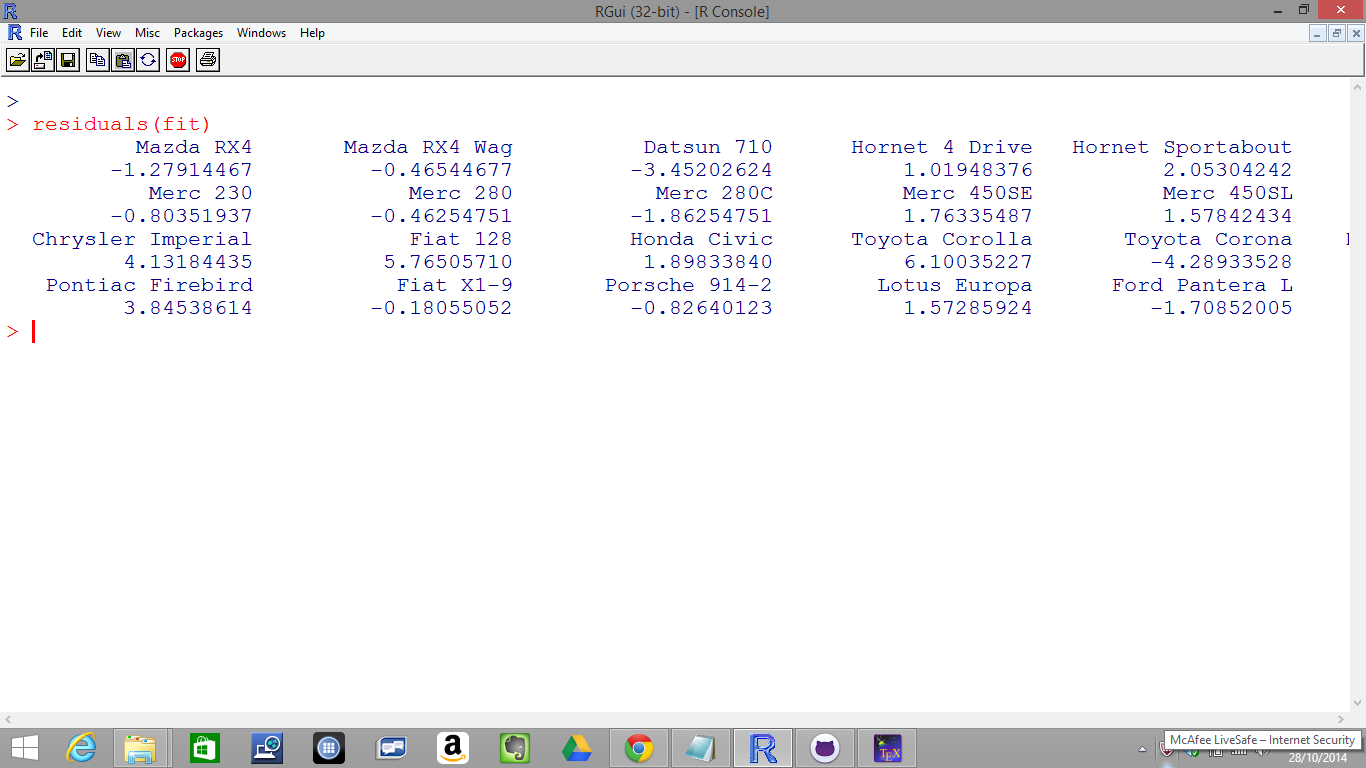
\includegraphics[width=0.9\linewidth]{screenshot1}
\caption{}
\label{fig:screenshot1}
\end{figure}
\begin{verbatim}
> sum(residuals(fit))
[1] 1.096345e-15

> #Shapiro-Wilk Test for Normality
> shapiro.test(resid(fit))
 
 Shapiro-Wilk normality test
 
 data:  resid(fit)
 W = 0.9375, p-value = 0.06341
 
 
\end{verbatim}

\end{document}